\documentclass[conference]{IEEEtran}
\IEEEoverridecommandlockouts
% The preceding line is only needed to identify funding in the first footnote. If that is unneeded, please comment it out.
%Template version as of 6/27/2024

\usepackage{cite}
\usepackage{amsmath,amssymb,amsfonts}
\usepackage{algorithmic}
\usepackage{graphicx}
\usepackage{textcomp}
\usepackage{xcolor}
\usepackage{float}
\def\BibTeX{{\rm B\kern-.05em{\sc i\kern-.025em b}\kern-.08em
    T\kern-.1667em\lower.7ex\hbox{E}\kern-.125emX}}
\begin{document}

\title{Model simulation of an orbit with an internally moving mass\\
}

\author{
\IEEEauthorblockN{Lukas Ehlers} \\
\IEEEauthorblockA{\textit{UiT The Arctic University of Norway} \\
\textit{Department of Computer Science} \\
Tromsø, Norway }
}

\maketitle

\begin{abstract}
    TODO abstract
\end{abstract}

\begin{IEEEkeywords}
    todo,todo
\end{IEEEkeywords}

\section{Einleitung}

Die Lebensdauer moderner Satelliten wird maßgeblich durch die verfügbare Menge an Treibstoff bestimmt. Dieser wird nicht nur für Bahnmanöver und Kurskorrekturen benötigt, sondern oft auch zur Stabilisierung und Lagekontrolle. Ist der Treibstoff aufgebraucht, endet in vielen Fällen der operative Betrieb, obwohl alle anderen Systeme weiterhin funktionsfähig wären.

Vor diesem Hintergrund wird nach alternativen Methoden gesucht, um Steuerungs- oder Bahnbeeinflussungseffekte ohne aktiven Treibstoffverbrauch zu realisieren. Eine vielversprechende Idee besteht darin, interne Masseverlagerungen gezielt zu nutzen, um über Trägheits- und Gravitationseffekte die Bahn oder Ausrichtung eines Satelliten zu beeinflussen. In dieser Arbeit wird untersucht, welchen Einfluss die Position einer beweglichen internen Masse auf den Orbit eines Körpers im Gravitationsfeld eines Zentralkörpers hat.

\section{Theoretische Grundlagen}

Die physikalische Grundlage der vorliegenden Untersuchung beruht auf mehreren zentralen Prinzipien der klassischen Mechanik. Zunächst gilt in einem abgeschlossenen System ohne äußere Kräfte das \textit{Gesetz der Impulserhaltung}: Der Gesamtimpuls bleibt konstant, selbst wenn sich Massen innerhalb des Systems bewegen \cite{goldstein}. Dies bedeutet, dass die Verschiebung einer internen Masse -- etwa durch einen Elektromotor innerhalb eines Zylinders -- den Gesamtschwerpunkt des Systems nicht verändert, solange keine äußere Kraft wirkt.

Darüber hinaus bewegt sich der Schwerpunkt eines ausgedehnten Körpers in einem Gravitationsfeld so, als wäre die gesamte Masse in diesem Punkt konzentriert \cite{taylor, landau}. Dies erlaubt es, die Bahn des Systems zu berechnen, ohne die interne Massenverteilung direkt berücksichtigen zu müssen, solange das äußere Feld näherungsweise als zentral betrachtet werden kann.

Ein zentrales Ergebnis ist, dass innere Massenverlagerungen die Bahn eines abgeschlossenen Systems im Gravitationsfeld nicht beeinflussen, sondern lediglich dessen Rotationsdynamik ändern können. Dies ist in der Raumfahrttechnik bekannt, etwa bei Satelliten mit Reaktionsrädern oder verschiebbarem Treibstoff \cite{marion}.

Schließlich liefert das \textit{Noether-Theorem} eine tiefere theoretische Begründung: Es stellt den Zusammenhang zwischen Symmetrien und Erhaltungsgrößen her. So führt Translationssymmetrie zur Impulserhaltung, Rotationssymmetrie zur Erhaltung des Drehimpulses \cite{noether}.




\section{Gravitationskraft}

Die Gravitationskraft auf ein Objekt mit Masse \( m \) im Feld eines zentralen Körpers mit Masse \( M \) ergibt sich zu:

\[
\vec{F}_\text{grav} = -G \cdot \frac{M \cdot m}{r^2} \cdot \hat{r}
\]

Dabei ist:
\begin{itemize}
  \item \( G \): Gravitationskonstante
  \item \( M \): Masse des Zentralkörpers
  \item \( m \): Masse des umlaufenden Körpers (Zylinder + Gewicht)
  \item \( r \): Abstand zwischen dem Schwerpunkt des Körpers und dem Zentrum
  \item \( \hat{r} \): Einheitsvektor vom Schwerpunkt zum Zentralkörper
\end{itemize}


\section{Ansatz bewegliches Gewicht}

\begin{figure}
    \centering
    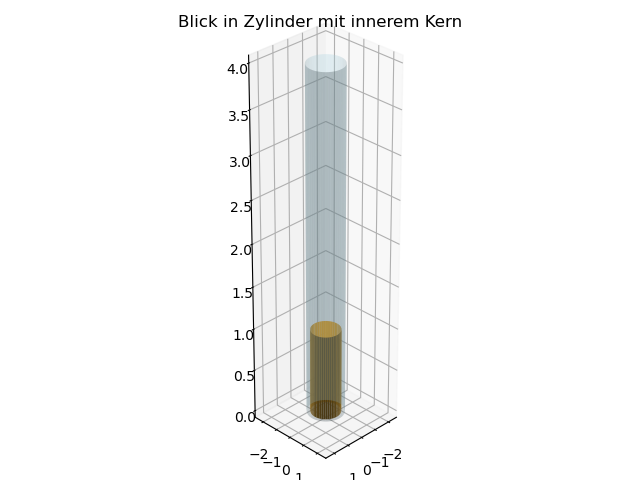
\includegraphics[width=\linewidth]{pics/sat_model_abstract/plot.png}
    \caption{Model bewegliches Gewicht}
    \label{fig:abstract_model}
\end{figure}


Die Abbildung~\ref{fig:abstract_model} zeigt ein vereinfachtes Modell eines rotationssymmetrischen Körpers, bestehend aus einem größeren äußeren Zylinder, der einen kleineren, beweglichen Innenzylinder enthält. In der schematischen Darstellung sind lediglich die geometrischen Grundstrukturen wiedergegeben. Nicht sichtbar ist der technische Mechanismus zur Verlagerung der inneren Masse: Der Innenzylinder ist auf einem Gewinde gelagert und kann entlang der Zylinderachse verschoben werden. Die Verschiebung erfolgt durch einen kompakten Elektromotor, der ohne konventionellen Treibstoff auskommt. Stattdessen wird der Motor ausschließlich durch Sonnenenergie betrieben, welche über am äußeren Zylinder montierte Solarzellen aufgenommen und in elektrische Energie umgewandelt wird.


\section{Schwerpunkt des Systems}
Das Gesamtsystem besteht aus:
\begin{itemize}
  \item Zylinderhülle mit Masse \( m_\text{body} = 9 \)
  \item Bewegliches Gewicht mit Masse \( m_\text{payload} = 1 \)
\end{itemize}

Die Schwerpunktposition ergibt sich zu:

\[
\vec{r}_\text{cm} = \frac{m_\text{body} \cdot \vec{r}_\text{body} + m_\text{payload} \cdot \vec{r}_\text{payload}}{m_\text{body} + m_\text{payload}}
\]

\subsection*{Fall: Gewicht weiter entfernt vom Planeten}

Gegeben:
\[
\vec{r}_\text{body} = (10, 0), \quad \vec{r}_\text{payload} = (11, 0)
\]

Dann:
\[
\vec{r}_\text{cm} = \frac{9 \cdot (10, 0) + 1 \cdot (11, 0)}{10} = (10.1, 0)
\]

\section{Gravitationskraft auf den Schwerpunkt}

Zentralmasse: \( M = 1000 \), Gesamtmasse: \( m = 10 \), Abstand: \( r = 10.1 \)

\[
\vec{F} = - G \cdot \frac{M \cdot m}{r^2} \cdot \frac{\vec{r}_\text{cm}}{r}
= - \frac{1000 \cdot 10}{10.1^2} \cdot \frac{(10.1, 0)}{10.1}
\]

\[
= - \frac{10000}{102.01} \cdot (1, 0) \approx -98.03 \cdot (1, 0) = (-98.03, 0)
\]

\section{Beschleunigung}

\[
\vec{a} = \frac{\vec{F}}{m} = \frac{(-98.03, 0)}{10} = (-9.803, 0)
\]

\section{Numerische Integration (Euler-Verfahren)}

\begin{align*}
\vec{v}_\text{neu} &= \vec{v} + \vec{a} \cdot \Delta t = (0, 3.0) + (-9.803, 0) \cdot 0.01  \\
\vec{v}_\text{neu} &= (-0.098, 3.0) \\
\vec{r}_\text{neu} &= \vec{r} + \vec{v}_\text{neu} \cdot \Delta t = (10.0, 0.0) + (-0.098, 3.0) \cdot 0.01 \\
\vec{r}_\text{neu} &=(9.99902, 0.03)
\end{align*}


\section{Simulation}

\begin{figure}[H]
    \centering
    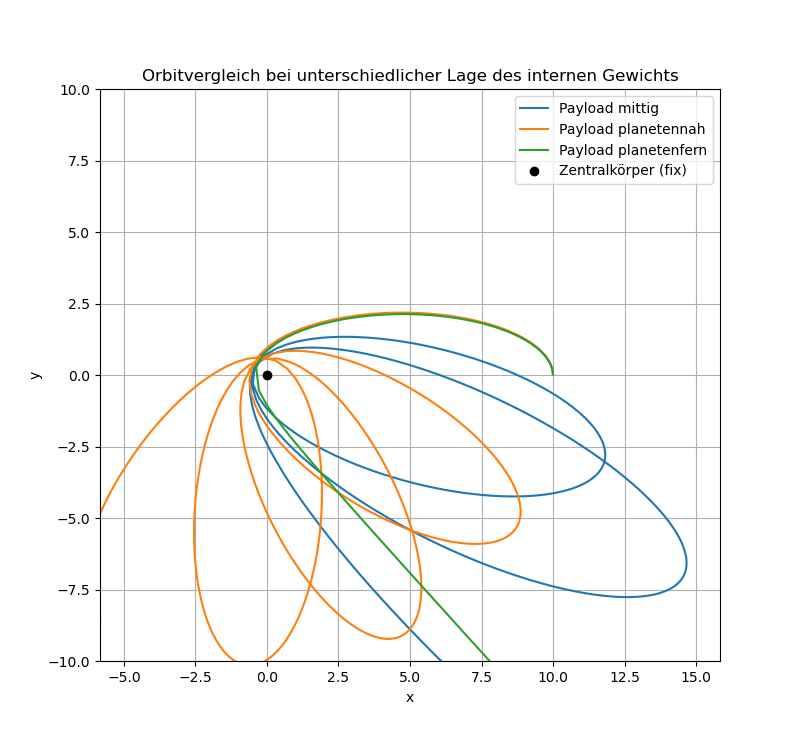
\includegraphics[width=\linewidth]{pics/orbits.png}
    \caption{unterschiedliche Orbits je nach Lage der Masse}
    \label{fig:orbits}
\end{figure}

Die in Abbildung~\ref{fig:orbits} dargestellten Trajektorien zeigen deutlich, dass sich die Umlaufbahn des Körpers in Abhängigkeit von der Lage der internen Masse leicht verändert. Obwohl sich die Gesamtmasse des Systems nicht ändert, führt die Verlagerung des Schwerpunkts zu veränderten Anfangsbeschleunigungen und infolgedessen zu unterschiedlichen Bahnverläufen.

Besonders auffällig ist die Bahn bei planetennaher Position des Gewichts (orangefarbene Kurve): Diese weist stärkere Bahnkrümmungen auf, was auf höhere Gravitationsbeschleunigungen bei näherem Schwerpunkt zurückzuführen ist. Die Bahn wirkt instabiler und oszilliert stärker, was über längere Zeiträume zu einer merklich anderen Umlaufdynamik führen kann.

Im Gegensatz dazu zeigt die grüne Kurve (Gewicht planetenfern) einen etwas flacheren und stabileren Orbit mit größerem Apogäum. Der Schwerpunkt liegt hier weiter vom Zentralkörper entfernt, was die Gravitationskraft reduziert und somit die Bahn weitet.

Die mittlere Konfiguration (blau) dient als Referenz. Sie zeigt einen symmetrischeren Orbit, da hier der Schwerpunkt des Systems mit dem geometrischen Mittelpunkt des Zylinders übereinstimmt.

Diese Resultate zeigen, dass bereits kleine Variationen der internen Masseverteilung zu langfristig signifikanten Unterschieden im Bewegungsverlauf führen können, was insbesondere für präzise Navigation oder Bahnkontrolle von Bedeutung ist – etwa bei Satelliten mit beweglicher interner Masse (z.\,B. Treibstoffverlagerung, mobile Nutzlasten).


\subsection{Numerische Simulation der Satellitenbewegung}
-LINK ZU GITHUB MIT CODE-

Die Simulation der Satellitenbewegung basiert auf dem Gravitationsgesetz von Newton, mit dem die Gravitationskraft zwischen Erde und Satellit bestimmt wird. Zur Integration der Bewegung über die Zeit wird das klassische Runge-Kutta-Verfahren verwendet, welches sich durch hohe Genauigkeit bei der numerischen Berechnung von Position und Geschwindigkeit auszeichnet. In jedem Zeitschritt werden die aktuellen Positions- und Geschwindigkeitswerte des Satelliten mithilfe dieser Methode aktualisiert, sodass sich über die Zeit eine Bahn ergibt, die anschließend visualisiert wird.


\section{Fazit}

Durch die wiederholte Anwendung von:
\begin{itemize}
  \item Schwerpunktberechnung
  \item Gravitationskraft auf den Schwerpunkt
  \item Integration der Bewegung (Position, Geschwindigkeit)
\end{itemize}
ergibt sich die Bahn des Körpers. Verschiebt sich der interne Schwerpunkt (z.\,B. durch Bewegung der Masse), beeinflusst dies leicht die Bahn – besonders über viele Umläufe hinweg.

\begin{thebibliography}{9}

\bibitem{goldstein}
Goldstein, H., Poole, C. P., \& Safko, J. L. (2002). \textit{Classical Mechanics} (3rd ed.). Pearson.

\bibitem{taylor}
Taylor, J. R. (2005). \textit{Classical Mechanics}. University Science Books.

\bibitem{landau}
Landau, L. D., \& Lifshitz, E. M. (1976). \textit{Mechanics}. Elsevier.

\bibitem{marion}
Marion, J. B., \& Thornton, S. T. (2003). \textit{Classical Dynamics of Particles and Systems} (5th ed.). Brooks Cole.

\bibitem{noether}
Noether, E. (1918). Invariante Variationsprobleme. \textit{Nachrichten von der Gesellschaft der Wissenschaften zu Göttingen, Mathematisch-Physikalische Klasse}, 235--257.

\end{thebibliography}


\end{document}
